\chapter{正则化方法}

\section*{Introduction}
	本章节内容主要介绍机器学习、深度学习总的正则化方法
	
	一般来说,所有的监督学习都可以最小化下面的函数来表示:
	
	\begin{equation}
		w = \arg \min_{w} \sum_{i}L(y_i,f(x_i;w)) + \lambda \Omega(w)
	\end{equation}
	
	其中,第一项一般为模型预测的结果与真实的结果之间的差距,可以用各种各样不同的函数来表示,第二项一般为正则化项,主要目的是使我们的模型更加简单,防止过拟合。

\section{L1 L2}
	\boldmath  %公式加粗
	
	\subsection{ill-condition}
	我们都知道优化问题有两大难题。一个是局部最小值的问题:我们要找的是全局最小值,如果局部最小值太多,那我们的优化算法就很容易陷入局部最小而不能自拔。另外一个就是ill-condition的问题。加入我们有个方程组$Ax=b$,我们要做的是求解$x$,如果$A$或者$b$稍微的改变,会使得$x$发生很大的变化,那么这个方程组系统就是ill-condition的,反之就是well-condition的。
	
	\begin{figure}[htbp]
	\centering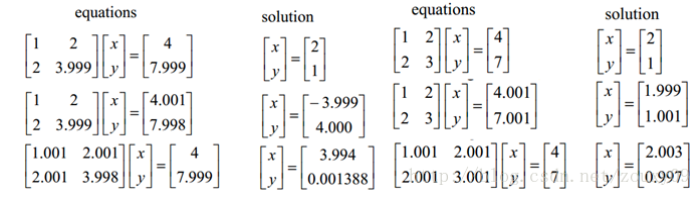
\includegraphics[width=6in]{img/3-1.png}
	\caption{ill-condition}\label{fig:3-1}
	\end{figure}
	
	第一行我们假设$Ax=b$,第二行我们稍微改变下$A$,结果的变化就非常大,第三行我们稍微改变下$b$,结果的改变同样是非常大的,因此我们可以认为我们的模型对错误的容忍力太低了,即对误差太敏感了。那么对于数据中难免存在的误差来说,模型的效果就非常差。
	
	因此我们需要一个指标去衡量ill-condition问题中的变化问题。
	
	condition number 衡量的就是在输入发生微小改变的时候,输出会发生多大的变化。也就是对系统微小变化的敏感度。condition number比较小(在1附近)的就是well-condition的,比较大的(远大于1的)就是ill-condition的。
	
	另外如果使用迭代优化的算法,当condition number太大的时候,会拖慢迭代的收敛速度。
	
	\subsection{L1}
	L1 norm 就是绝对值的和,公式如下
	
	$\|x\|_p = |x_1|+|x_2|+...+|x_n|$
	
	\subsection{L2}
	L2 norm 就是我们经常说的欧几里得范数,公式如下
	
	\begin{equation}
		\|x\|_2 = (\sum_{i=1:n}x_i ^{p})^{\frac{1}{p}}
	\end{equation}
	
	caffe中weight decay 这个参数代表L2范数前的系数。
	
	L2的优点:
	\begin{itemize}
		\item 可以防止过拟合,提升模型的泛化能力
		\item L2范数有助于处理condition number不好的情况下逆矩阵求逆很困难的情况(待定)。
	\end{itemize}

	
	
	\subsection{L1与L2的不同}
	对于L1和L2规则化的代价函数来说,我们可以写成如下的形式
	
	\begin{equation}
		Lasso:\min_{w} \frac{1}{n} \|y-Xw\|^2,s.t.\|w\|_1<=C
	\end{equation}
	
	\begin{equation}
		Ridge:\min_{w} \frac{1}{n} \|y-Xw\|^2,s.t.\|w\|_2<=C
	\end{equation}
	
	为了便于可视化,我们考虑两维的情况,在$(w_1,w_2)$平面上画出目标函数的等高线,而约束条件则成为平面上半径为C的一个norm ball。等高线与norm ball相交的地方就是最优解:
	
	\begin{figure}[htbp]
	\centering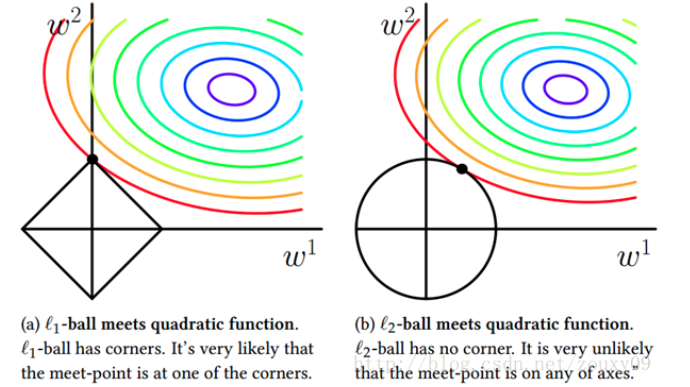
\includegraphics[width=6in]{img/3-2.png}
	\caption{图}\label{fig:3-2}
	\end{figure}
	
	可以看到,在相交的地方,L1在和每个坐标轴相交的地方都有出现解,即更容易出现$w_1$或者$w_2$为0的解,可以用来提取特征,更加容易产生稀疏性。
	
	L2的话更容易出现$w_1$和$w_2$都不是0的情况,虽然有时候会出现很小的值。在更高维的情况下也是这样的,即基本上只是用来正则化而已。
	
	
	
	
	
	
	
	
	
	
	
	
	
	
	
	
	
	
	